\section{RGB Loco-Manipulation via Teacher-Student-Bootstrap}
\label{sec:method}



% In this section, we present the setup of \method{} on top of classical teacher-student distillation literature. We first describe the large-scale synthetic generation pipeline for physically realistic and visually stunning door scenes in IsaacLab~\cite{isaaclab2025}. We then discuss the additional design choices, such as a multi-staged exploration encouragement scheme tailored for long-horizon loco-manipulation tasks, and a bootstrapping approach to overcome the partial observability issue of student policies.

Here we present \method{}'s three-phase training, building on classical teacher–student distillation. We first outline a visual sim-to-real pipeline for whole-body loco-manipulation, emphasizing two design elements: a multi-stage exploration scheme tailored to long-horizon tasks and a bootstrapped refinement strategy that mitigates partial observability in the student. We then describe a large-scale synthetic generation pipeline in IsaacLab~\citep{isaaclab2025} that produces physically realistic and visually diverse door environments for training and evaluation, treating door opening as a representative loco-manipulation task.

\subsection{Visual RL and Teacher-Student Distillation}

\minisection{Preliminary} Consider a partially observable Markov decision process (POMDP) $\mathcal{P} = (\mathcal{S}, \mathcal{A}, \mathcal{O}, T, \mathcal{R}, \mathcal{O}, \gamma, \rho_0)$, where $\mathcal{S}$ is the state space, $\mathcal{A}$ the action space, $\mathcal{O}$ the observation space, $T(s'|s,a)$ the transition kernel, $\mathcal{R}(s,a)$ the reward, $\mathcal{O}(o|s)$ the observation, $\gamma\in[0,1)$ the discount factor, and $\rho_0$ the initial state distribution. In humanoid whole-body control literature, the policy is responsible for outputting target joint positions, which, in the case of a Unitree G1 robot, includes 29 body joints and 14 hand joints, resulting in an extremely high action space dimension of 33. These joint angles are then tracked by low-level motors using a PD control law. Contrary to quasi-static manipulation literature, the policy needs extremely meticulous reasoning of torque-level dynamics to balance the robot, especially when pushing against a spring-loaded door. The policy also needs to be inferenced consistently at \SI{50}{\hertz}, which requires efficient neural network architectures. We build \method{} on top of a pretrained whole-body controller \citep{ben2025homie} to alleviate the extra burden of handling legged locomotion from scratch.

\minisection{Teacher Policy} The teacher policy $\pi_T(a|s)$ at time $t$ has access to privileged information $o_T\in\mathcal{O}$ that are typically not directly available outside simulation. These include ground-truth robot-root-to-door transform $\xi_\text{RD}$, left-hand- and right-hand-to-door-handle transform $\xi_\text{LD}, \xi_\text{RD}$, net contact wrenches on the 18 hand bodies $\tau_H \in \mathbb{R}^{18 \times 6}$, and root linear velocity $v_R \in \mathbb{R}^3$. While previous works estimate some of these quantities using a hard-coded estimator~\citep{traverse-doors-2025,xiong2024adaptive,calvert2025behavior}, our goal is to eliminate such priors at deployment and maximize generalization with a pure RGB–based student. We train the teacher policy using standard proximal policy optimization (PPO)~\citep{schwarke2025rslrl}, with the exact reward shaping recipe available in Appendix \ref{app:teacher-reward}.

 \minisection{Student Distillation} While the student policy has access to non-privileged proprioception information, such as joint angles $q$, joint velocities $\dot{q}$, and root angular velocities $\dot{\omega}\in\mathbb{R}^3$, its perception of the task relies mostly on the input RGB observation and its temporal context. The image is processed by a vision encoder~\citep{resnet2015}, and the resulting latent is concatenated with the proprioceptive features and passed through a two-layer LSTM (512 units each). A three-layer MLP (512, 256, 128) then maps the recurrent features to target joint angles. The vision encoder is jointly fine-tuned with the policy. The student is interactively distilled using DAgger~\citep{ross2011dagger}, which enables direct supervision on the student's input distribution, compared to behavioral cloning which only covers the teacher distribution.

% \minisection{Simulation Considerations}

\subsection{Multi-Stage Whole-Body Loco-Manipulation}

\begin{figure*}
    \centering
    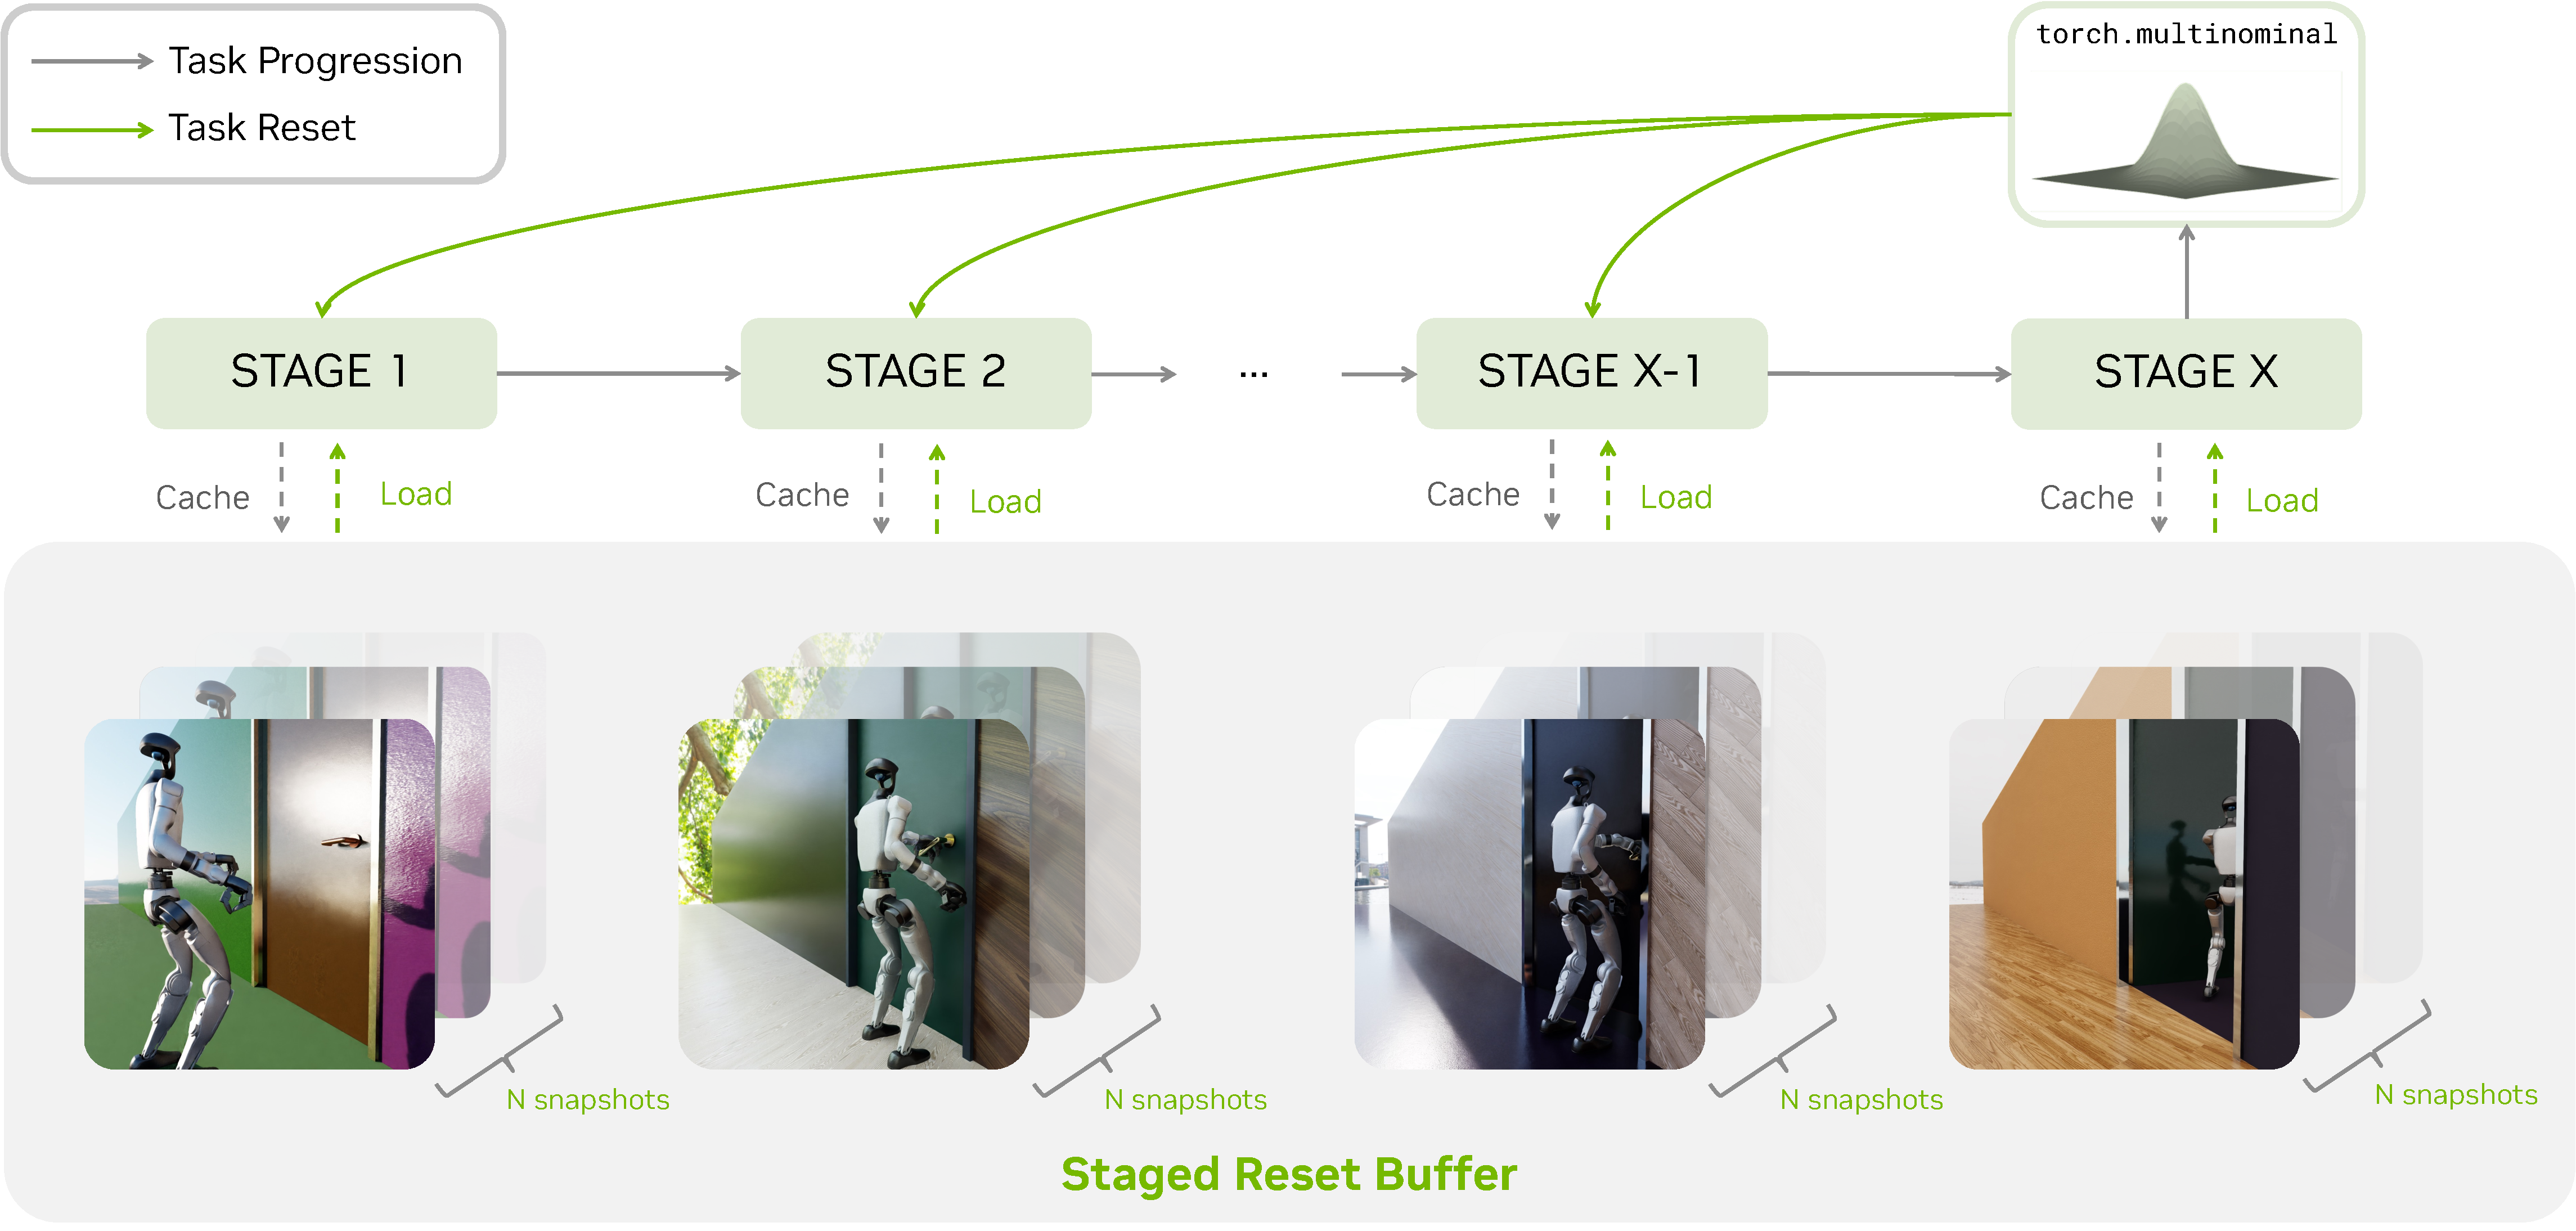
\includegraphics[width=\linewidth]{figs/drafts/fig_staged_reset.pdf}
    \caption{Overview of the staged-reset exploration scheme. When entering a new stage, a snapshot of the simulation is cached into the buffer. When the task resets, the environment is randomly reset to a prior stage by loading from the cache.}
    \label{fig:staged-reset}
\end{figure*}

Here, we present the design of a robust teacher training pipeline for whole-body loco-manipulation tasks. Similar to~\citet{wococo2024}, we design a stage-based reward system to decompose the task into atomic stages, each with its own reward formulations. We inject certain inductive human bias, such as using the door handle and hinge state to distinguish between the approaching, opening, and traversing stages of a successful door-opening operation.

We find that contact-rich tasks that require precise manipulation, such as using articulated doors, present unique challenges in encouraging steady exploration and advancements into later stages. These challenges have not been foreseen in the prior success of RL whole-body control literature. Intuitively, grasping a door handle without the knowledge of carefully rotating it in the correct direction or pairing with precise whole-body movement would incur additional penalties due to the excessive use of motor torque, peaking contact forces, or even the risk of falling over, causing the policy to ``unlearn'' the grasping behavior and keep away from advancing to the next stage.

To improve training efficiency, inspired by~\citet{first_return2021}, we design a simple exploration encouragement scheme leveraging the full recoverability of physical simulators. When an environment proceeds to the next stage, a rolling buffer keeps the recent 100 snapshots of the robot and environment (the door) at that step, which includes the generalized coordinates of all articulated and rigid objects in the scene. Then at reset time, the robot is randomly reset to either the initial stage or one of the middle stages under a nonzero probability. This pipeline is illustrated in Figure \ref{fig:staged-reset}.

To formulate it more formally and clearly see its effect in on-policy RL, consider a long-horizon, multi-stage task, for instance, approaching the door (Stage 1) and opening it (Stage 2). These stages correspond to disjoint subsets $\{S_1,\dots,S_K\} \in S$ connected by narrow transitional regions or bridges $\mathcal{B}_{y,y+1} \in S_y$ that must be traversed to reach the next stage. Because exploration across such bridges has very low probability $p_{\text{bridge}} \ll 1$, policies trained from $\rho_0$ often fail to reach downstream stages early in training, yielding poor long-horizon credit assignment.

To address this, we introduce a \textbf{staged reset law}
\begin{equation}
    \alpha = (\alpha_1, \dots, \alpha_K), \quad \sum_{y=1}^K \alpha_y=1,
\end{equation}
which specifies the fraction of rollouts initialized from each stage's reset distribution $\rho_y$. The resulting initial distribution therefore becomes
\begin{equation}
    \tilde{\rho}_\alpha = \sum_{y=1}^K \alpha_y \rho_y
\end{equation}
with an updated discounted occupancy measure
\begin{equation}
    d_\pi^\alpha(s)=(1-\gamma)\sum_{t=0}^\infty \gamma^t \text{Pr}(s_t=s \vert s_0 \sim \tilde{\rho}_\alpha, \pi),
\end{equation}
where $\text{Pr}$ denotes marginal probability. This shows that the staged-reset scheme reweighs the occupancy measure towards later-stage regions, increasing the frequency and effective magnitude of gradient updates for those states. 




\subsection{RL Finetuning for Partial Observability}

In teacher–student policy distillation, a student policy $\pi_S(a|o)$ receives only partial observations $o_t\in\mathcal{O}$, while the teacher policy $\pi_T(a|s)$ has access to privileged observations. Standard behavioral cloning loss alone may not yield optimal performance when the student observation space omits key features due to occlusion. In practice, the student policy often needs to bootstrap on its own rollouts to discover additional strategies that compensate for its partial observability, such as adjusting the robot's position so the manipulated region remains in the camera's field of view.

To enable this self-improvement, we fine-tune the student policy with a Group Relative Policy Optimization (GRPO) \citep{grpo2024} algorithm, which is an actor-only variant of PPO that omits the value function and instead estimates baselines from grouped trajectory scores. Let a batch of $G$ rollouts $\{\tau_i\}_{i=1}^G$ be sampled from the current policy $\pi_S$, each with return $R_i$. We define normalized group-relative advantages
\begin{equation}
    \hat{A}_i = \frac{R_i - \text{mean}(R)}{\text{std}(R)},
\end{equation}
and update $\pi_S$ using the clipped PPO surrogate:
\begin{equation}
    \mathcal{L}_{\text{GRPO}}(\theta) = \Exp{i,t}{\min(r_{i,t}(\theta)\hat{A}_i, \\ \text{clip}(r_{i,t}(\theta), 1-\epsilon, 1+\epsilon)\hat{A}_i},
\end{equation}
where $r_{i,t}(\theta)=\frac{\pi_\theta(a_{i,t}|o_{i,t})}{\pi_\text{old}(a_{i,t}|o_{i,t})}$.

Conceptually, this GRPO fine-tuning phase allows the student to improve beyond imitating the teacher, optimizing its behavior directly under its own partial observations.
Empirically, we observe that such bootstrapping leads the vision-based student to learn compensatory behaviors that the teacher never demonstrated, such as keeping manipulated objects centered in view or adjusting end-effector poses to maintain visibility.
Thus, GRPO acts as a lightweight, stable reinforcement refinement phase that complements behavior cloning, bridging the gap between imitation from privileged demonstrations and robust autonomous performance.

It is worth mentioning that during fine-tuning, we use mainly a binary task success signal, plus simple shaping reward terms such as joint velocity, joint acceleration, and action rate penalty to regularize the humanoid behavior. Therefore, this approach can be a drop-in solution to improve any loco-manipulation task with a base policy of non-zero success rate.


\subsection{Massive-Scale Simulation Randomization}

\begin{figure*}
    \centering
    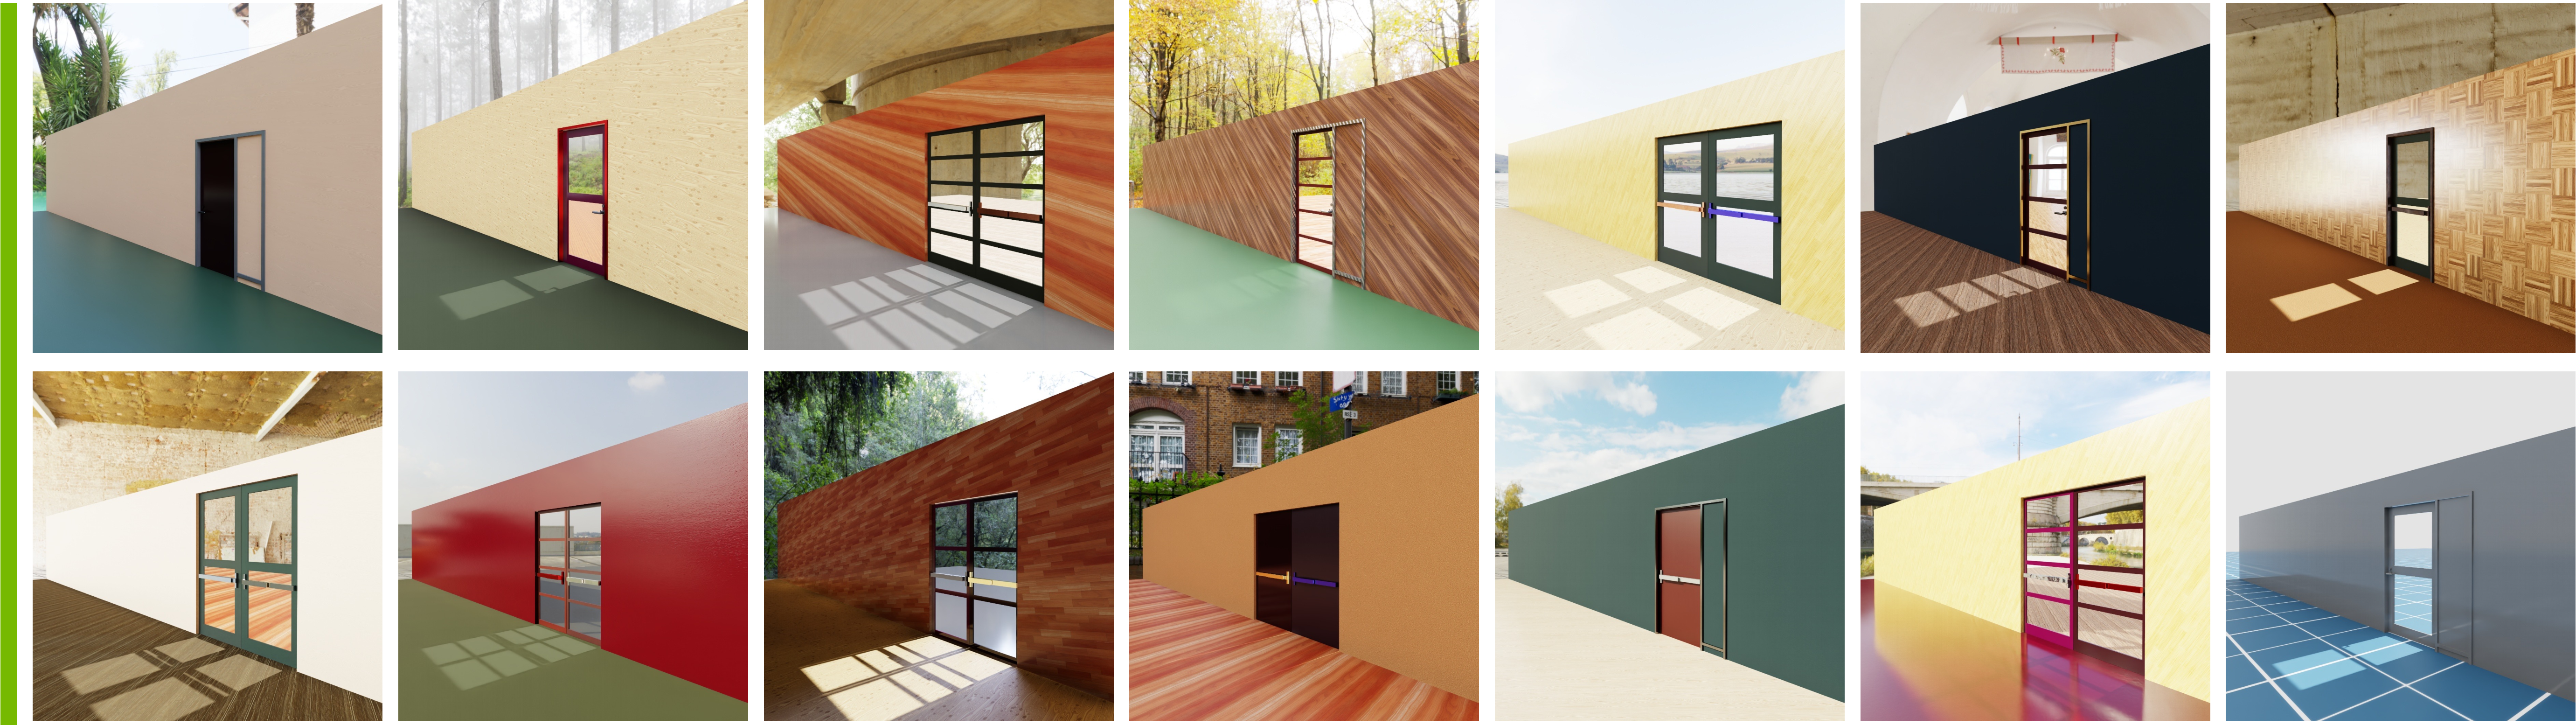
\includegraphics[width=\linewidth]{figs/drafts/fig_sim_doors.pdf}
    \caption{Procedurally generated doors used to train \method{}, covering panel designs, latching mechanisms, lighting, materials, etc. Each parallelized environment is trained on a unique set of door parameters. The last figure shows a door without material.}
    \label{fig:sim-doors}
\end{figure*}

To scale the visual and dynamics diversity of our whole-body loco-manipulation task to an unprecedented level, we design a procedural generation pipeline in IsaacLab that spawns physically and visually diverse yet realistic articulated assets. Compared with prior work such as Infinigen-Sim~\citep{ifinigensim2025}, our IsaacLab-native implementation significantly improves physical realism and enables contact simulation that is both accurate and efficient for parallel RL workflows.

\textit{We emphasize that we do not re-create real-world scenes in simulation; rather, all real-world scenes we evaluate in are unseen during training}. The procedural generation pipeline does not bias towards the specific dimension, physical response, texture, color, or lighting of any real-world location. This contrasts with small-scale behavioral cloning literature~\citep{lee2025stageact} that is confined to be evaluated on the exactly same scene, background, lighting, and time-of-day which the data were originally collected.

\minisection{Physical Variations} We include 5 different door types in the generation pipeline covering commonly seen doors in 3 broad categories: pushing door with rotational handle; pulling door with rotation handle; pushing door with push bar. Similar to~\citet{traverse-doors-2025}, all conceivable aspects of the physical properties of the doors are randomized, such as door dimension, handle location, door-hinge damping, and door-handle resistive torque. Most notably, realistic latching mechanism is used to capture the abrupt change in whole-body dynamics at the moment of opening.

\minisection{Visual Variations} Random textures are drawn from IsaacLab's Physically Based Rendering (PBR) materials and applied to all surfaces. In addition, 5233 dome-light textures are applied to simulate various locations and times of day. To balance rendering quality and performance while training an RL policy in parallel, we use the RTX Real-Time renderer in performance mode, with post-processing effects such as motion blur and auto white balance enabled. Camera extrinsics and intrinsics are aligned and slightly randomized. These settings are essential for re-creating harsh real-world correspondence with the camera being mounted on a legged robot under constant contact switching.